%
% On a majoré avec ce rapport ;-)
%

\documentclass[a4paper,11pt]{article}

\usepackage[utf8]{inputenc}
\usepackage[T1]{fontenc}
\usepackage{lmodern}
\usepackage{amsmath}
\usepackage{amssymb}
\usepackage{amsthm}
\usepackage{textcomp}
\usepackage{wasysym}
\usepackage[top=2.2cm, bottom=2cm, left=2.2cm, right=2.2cm]{geometry}
\usepackage{graphicx}
\usepackage[svgnames,table]{xcolor}
\usepackage{tikzsymbols}
\usepackage{longtable}
\usepackage{listings}
\usepackage{eurosym}
\usepackage{float}
\usepackage{enumerate}
\usepackage{wrapfig}
\usepackage[francais]{babel}

\theoremstyle{remark}
\newtheorem*{rem}{\textcolor{Teal}{Remarque}}

\newcommand\R{\mathbf{R}}
\newcommand\N{\mathbf{N}}
\newcommand\C{\mathbf{C}}
\newcommand\Q{\mathbf{Q}}
\newcommand\Z{\mathbf{Z}}
\newcommand\E{\mathcal{E}}
\newcommand{\abs}[1]{\left\lvert#1\right\rvert}

\DeclareMathOperator{\argmax}{arg\ max}
\DeclareMathOperator{\sgn}{sgn}

\newcommand{\intervalle}[4]{\mathopen{#1}#2\mathclose{}\mathpunct{};#3\mathclose{#4}}
\newcommand{\intiff}[2]{\intervalle{[\![}{#1}{#2}{]\!]}}

\renewcommand*\rmdefault{ppl}

\usepackage[colorlinks=true,linkcolor=purple]{hyperref}


\begin{document}

\renewcommand{\contentsname}{Sommaire}
\setcounter{tocdepth}{1}

%%%%%%%%%%%%%%%%%
% Page de titre %
%%%%%%%%%%%%%%%%%


\begin{titlepage}
	\newcommand{\HRule}{\rule{\linewidth}{0.5mm}}

	\center

	\textsc{\LARGE Télécom ParisTech}\\[1.2cm]

	\HRule \\[0.8cm]
	{ \huge \bfseries SES 107}\\[0.4cm]
	{ \huge \bfseries Rapport du jeu d'entreprise}\\[0.4cm]
	{ \huge \bfseries Univers 1 : Les Procréateurs}\\[0.4cm]
	\HRule \\[1.4cm]
	
	{\large \today}\\[1.5cm]

	\begin{minipage}{0.4\textwidth}
	\large
	\emph{Groupe :}\\
	Anas \textsc{Barakat}\\
	Alexis \textsc{Bauvin}\\
	Marie \textsc{Déchelle Marquet}\\
	Alexandre \textsc{Poinso}\\
	Régis \textsc{Gourdel} \\
	\end{minipage}~\hspace{9.5cm}
	
	\vspace{1.2cm}

	\tableofcontents

	\vspace{2.5cm}

	\begin{figure}[htp]
	\centering
	
\includegraphics[scale=0.11]{./logoTelecom.png}
	\end{figure}


\end{titlepage}



\section{Présentation de la stratégie et des résultats}

	\subsection{Présentation au Conseil d’Administration}
	
		L’activité de notre entreprise a permis d’atteindre un retour cumulé aux actionnaires de 21,62\%, se hissant ainsi au 2\up{e} rang du marché de la  téléphonie mobile.
		Le résultat annuel a évolué de manière positive à partir de la 3\up{e} année grâce aux lancements progressifs de nouvelles technologies en accord avec la maturation des marchés et  l’augmentation des taux de couverture dans les différentes zones géographiques.
		Nous avons réalisé un résultat net de 575 millions de dollars à l’issue de cette dernière année fiscale.
		La figure présente l’évolution du résultat annuel sur les 7 dernières années.
		
		\begin{figure}[htp]
		\centering
		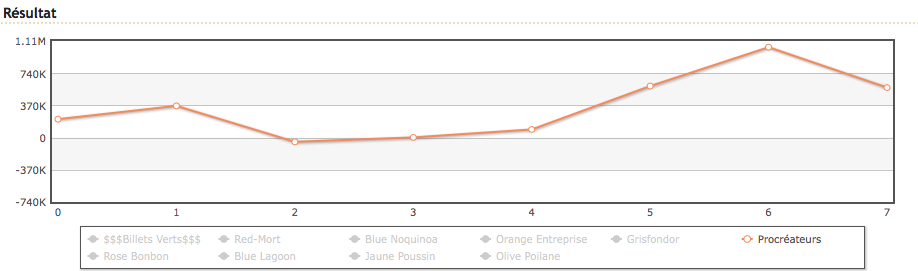
\includegraphics[scale=0.5]{./courbe_resultats.png}
		\end{figure}
		
		La stratégie de différenciation de l’entreprise privilégiant le haut de gamme et le High Tech a permis de s’imposer très vite sur le marché avec des prix permettant de dégager des marges importantes (jusqu’à 240\% la dernière année sur la technologie 4 en Europe), malgré la concurrence d’une entreprise arrivée à peine plus tôt sur le marché sur la même technologie.
		Le développement rapide de nouvelles technologies a été porté par un investissement conséquent sur la recherche et développement (jusqu’à 40\% des coûts la 2\up{e} année).
		Le retour sur investissement de cette opération s’est avéré fructueux à partir de la 3\up{e} année, suite aux lancements des nouveaux produits.  

		L’adaptation de l’offre aux différents marchés a permis d’optimiser les bénéfices.
		En effet, en proposant des téléphones de technologie de pointe en Europe, friande de high-tech, des technologies hybrides aux Etats-Unis et des technologies mois avancées en Asie avec des prix plus faibles, l’entreprise a généré des bénéfices dans toutes les zones géographiques. 
	
		Le versement de dividendes s’est fait sur le long terme pour influencer positivement le retour cumulé et pour augmenter le cours de l’action de l’entreprise sur les 2\up{e}, 5\up{e} et 7\up{e} années, et le rachat de 30 millions USD d’actions a permis de valoriser considérablement le cours de l’action de l’entreprise.
		Néanmoins, le remboursement de la dette durant les 2\up{e} et 3\up{e} année nous a empêché de verser des dividendes. 
	
		Nous tenons à remercier nos actionnaires pour la confiance qu’ils nous ont accordée en investissant dans notre entreprise.
		Notre situation financière actuelle positive nous permet de continuer d’investir dans de nouvelles technologies pour percer dans le marché dans la même lancée et en adoptant la même stratégie.
		L’orientation stratégique générale du groupe est donc maintenue.
	
	\subsection{Présentation aux représentants syndicaux de l’entreprise}
	
		Au cours de ces sept années passées en votre compagnie, notre groupe n'a cessé d'investir en Recherche et 	Développement afin d'être à la pointe de la technologie dans l'optique de capter le marché avant nos concurrents.
		Cette captation fut possible grâce à l'investissement de ce pôle, dans lequel nous avons procédé	à un recrutement intense avec des salaires attractifs, atteignant les 5 000 USD mensuels lorsque la concurrence moyennait à 4 700 USD.
		\mbox{}\\
 
		De plus, nous pouvons nous féliciter d'avoir une faible rotation de l'emploi, aux alentours de deux ou trois sur les années passées.
		Cette fidélisation du personnel montre que les employés se plaisent dans notre groupe, ce qui	crée un véritable esprit d'entreprise extrêmement propice à une ambiance d'innovation et d'efficacité.
		En effet, nous nous présentons comme l'un des groupes avec les employés les plus efficaces, ce dont nous vous félicitons, car témoin d'un intense désir de faire avancer l'entreprise.
		\mbox{}\\
		 
		Notre production est en majeure partie réalisée sur le sol Américain -- 12 usines au total -- afin de rester cohérent avec notre vision de Technologies 2 et 4 haut de gamme à destination du marché Européen, tandis qu'une faible partie de la production -- 4 usines -- est située sur le sol asiatique, où nous faisons produire des mobiles de Technologie 1 et 2 à moindre coûts pour des marchés plus modérés.
		Nous gardons ainsi le fleuron de notre technologie sur le sol de notre patrie.
		\mbox{}\\
 
		Cette stratégie a fini par porter ses fruits : bien que les trois premières années furent difficiles pour l'entreprise, les efforts combinés de tous nos ingénieurs furent efficaces. Les ventes de téléphones de technologie 4 furent très porteuses pour notre groupe, dont les bénéfices arrivèrent dès la 4\up{e} année.
		\mbox{}\\
		 
		Notre stratégie de recherche massive et de développement des nouvelles technologies, bien qu'efficace au début, connaît un certain déclin depuis l'arrivée de la concurrence.
		Cela nous a obligé à exprimer nos adieux	à certains de nos ingénieurs de Recherche et Développement, bien que leur licenciement fut effectué en douceur avec de beaux débouchés pour l'avenir.
		Cependant, la production devant être maintenue, toutes nos usines	furent conservées.
		\mbox{}\\
		 
		De plus, la production était faite quasiment intégralement en interne : la sous-traitance n'était utilisée qu'en dernier recours lorsque la demande soutenue excédait nos capacités de production -- au plus grand	avantage de nos ouvriers.
		Ceci a permis de maintenir de faible coûts de production et d'ouvrir toujours plus d'usines, en Asie notamment.
		Cette production interne démontre de votre qualité et de la confiance que	nous pouvons avoir dans nos ouvriers, qui ne se sentent pas remplacés par une main d'œuvre générique et délocalisée.
		\mbox{}\\
		 
		L'ensemble de ces décisions nous a permit d'établir une stratégie efficace et rentable, ayant participé à une forte création d'emplois, aussi bien d'ingénieurs de Recherche et Développement que d'ouvriers.
		Mais tout ceci n'aurait pas été possible sans la motivation et l'esprit d'innovation présent chez tous les employés du groupe.

\section{Analyse critique de la stratégie du groupe}

	\subsection{Stratégie et déroulé}

	% stratégie
	La stratégie qui a été adoptée dès le premier tour a consisté à miser sur les technologies 2 et 4 et viser de préférence un marché assez haut de gamme.
	
	La première technologie était également vendue mais à bas prix et avec peu de fonctionnalités, un positionnement nécessaire qui permettait de conserver une part de marché dans le low-cost sur les zones lentes à évoluer vers la technologie 4.
	La technologie 3 n'a pas du tout été développée afin de laisser notre offre s'articuler autour des deuxième et quatrième.
	
	En accord avec cette stratégie orientée haut de gamme, nous avons choisi des fournisseurs bien notés sur les plans de l'éthique et du développement durable et notre note sur ces deux points est restée assez bonne au cours de l'ensemble du jeu.
	
	\paragraph{}
	L'évolution de notre entreprise au cours des sept tours de jeu peut se résumer en trois phases que nous détaillons ci-après.

	\paragraph{} % première phase
	Dans un premier temps nous avons commencé à mettre en place notre stratégie de différenciation, en réalisant d'importantes embauches de personnel en recherche et développement notamment.
	Le maximum en effectifs a été atteint vers la fin de cette phase, au tour 3, avec 1100 personnes.
	Nous avons investi massivement sur les technologies 2 et 4.
	Nous avons par contre construit peu d'usines, toutes en Asie : une première au tour 2 et trois autres au tour 3.

	Les résultats obtenus ont alors été assez médiocres, la technologie 4 n'étant encore ni développée ni déployée.
	Toutefois les investissements dans la technologie 2 et les bonnes opportunités du marché pour son déploiement nous ont permis de commercialiser celle-ci à partir du troisième tour.
	Nos résultats ont donc commencé à remonter à partir de ce tour, notre offre étant particulièrement appréciée en Europe.
	Cela nous a permis de maintenir l'effort sur la recherche et de s'engager dans la phase suivante avec une avance technologique sur la technologie 4.

	\paragraph{}% seconde phase : bénéfices de la différenciation
	Dans un second temps nous avons pu retirer les bénéfices de cette stratégie de différenciation mise en place précédemment.
	Notre relative rapidité dans le développement de la technologie 4 nous a en effet permis de proposer un produit intéressant sur le marché européen, avec peu de concurrence, qui a été un moteur de notre croissance.
	Notre budget publicité a également été augmenté afin de vendre au mieux nos produits les plus évolués.
	Notre part de marché était en moyenne importante, et ce sur différentes technologies.
	
	Nous avons donc décidé de garder le cap fixé, étant alors la première entreprise mondiale de notre secteur, par le résultat et pour le retour cumulé.
	De plus nous avons stoppé les embauches en recherche et développement, diminuant légèrement nos effectifs sur chaque tour, car la marge de progression en termes d'innovation était dorénavant plus restreinte.
	La logistique a été optimisée pour fournir en priorité l'Europe, où nous avions le plus de dynamisme.

	C'est également à partir de cette période que nous avons commencé à reverser des dividendes, ainsi que, ponctuellement, à racheter des actions.

	\paragraph{} % dernière phase : ralentissement par manque de capacité de production
	Dans une dernière phase nous avons adapté notre marketing aux nouveaux impératifs du marché.
	L'impossibilité de continuer à innover nuisait en effet à la stratégie de différenciation que nous suivions.
	Pour maintenir des ventes rester compétitifs nous avons donc continué à ajouter des fonctionnalités, sans répercussion sur les prix.
	Les sociétés concurrentes possédaient des produits qui étaient alors aussi intéressants que les notre sur les technologies 2 et 4 et se livraient une guerre des prix.
	L'impossibilité de maintenir une avance technologique nous a donc conduit à nous insérer dans cette guerre des prix.

	Par rapport à la concurrence nous avons alors souffert de notre plus faible capacité de production, qui ne nous permettait pas d'avoir un coût unitaire assez bas.
	Nous avons donc essayé de compenser cela en maintenant un budget publicitaire assez élevé et en nous satisfaisant d'une part de marché moindre.

	Nous avons également réduit légèrement nos effectifs en recherche et développement.
	Ceux-ci étaient en effet très au-dessus de ceux de nos concurrents et ne se justifiaient plus au vu de la maturité du marché et du manque d'informations sur les futures technologies à déployer.
	Avec 900 ingénieurs nous restons la deuxième plus grosse entreprise par ses effectifs en R\&D.
	
	\subsection{Critique de la stratégie}

	Notre politique consistant à miser sur des produits haut de gamme avec une publicité importante s'est révélée efficace à moyen terme dans le jeu présenté.
	Nous avons pu grâce à cela prendre la tête sur plusieurs tours sur le marché, ce qui nous a fournit un avantage nous permettant d'assurer un résultat final correct.
	À plus long terme nous avons été pénalisé dans notre stratégie par le blocage dans l'innovation, et dans nos résultats par le fait d'avoir gardé un nombre élevé d'employés en R\&D, par fidélité à notre stratégie sans que cela ne nous apporte d'avantage concret à court terme.\\
	
	Une première difficulté que nous avons réussi à surmonter a été de ne pas laisser submerger par les dettes à court terme.
	Nous en avons en effet contracté alors que la technologie 4 n'était pas encore lancée et que nos revenus sur les technologies 1 et 2 étaient encore insuffisants.
	Mais celle-ci a rapidement été remboursée lorsque nos résultats se sont améliorés, grâce notamment aux bonnes ventes en Europe et en Asie, ainsi qu'un transfert d'argent depuis ces deux zones vers les USA pour résorber la dette dans ce pays.
	
	Une seconde difficulté dont nous avons plus souffert est l'adaptation de notre production à la demande.
	Au cours des première et dernière phase notre production était trop importante, nous laissant avec du stock, car nous n'étions pas alors suffisamment compétitifs.
	Au cours de la seconde phase ce fut l'inverse.
	La demande était plus importante et nous ne produisions pas assez pour y répondre.\\
	
	Enfin le jeu était tel qu'un investissement plus important dans des usines de production était nécessaire pour pouvoir mieux tirer sur les prix grâce à un coût unitaire moindre lorsque la pénurie d'innovation a égalisé les niveaux d'avancée technologique.
	C'est notamment une meilleure réussite sur ce point qui a permis à nos premiers concurrents de nous passer devant au cours des derniers tours.
	La croissance du secteur était assez importante sur les trois derniers tours, ce pourquoi nous avons du recourir de façon accrue à des sous-traitants.
	Or les prix de ceux-ci n'étaient pas suffisamment bas pour compenser l'absence de moyens de production propre de grosse capacité.\\
	
	Dans l'ensemble nous pensons que la stratégie mise en œuvre a fait ses preuves et aurait pu, dans la réalité, se révéler encore fructueuse à plus long terme.

\section{Questions}

	\subsection{Dans la réalité, la capacité d’innovation d’une entreprise dépend-elle d’autres éléments que du nombre de chercheurs en R\&D et de leur niveau de salaire, comme cela est modélisé dans le jeu ?}

		Dans la réalité, la capacité d'innovation d'une entreprise ne dépend pas que du nombre de chercheurs en R\&D et de leur niveau de salaire.
		En effet, le jeu ne prend pas en compte la probabilité d'échec d'un programme de R\&D comme ça l'est possible dans le monde réel.
		Dans le jeu, le temps passé et le nombre de chercheurs suffisent à débloquer de nouvelles fonctionnalités.
		Or, dans le monde réel, les recherches sont toujours incertaines.
		De plus, pour innover, une entreprise a d'autres solutions que celle de s'appuyer sur sa R\&D interne.
		Elle peut par exemple s'associer avec d'autres compagnies ou racheter des start-ups à fort potentiel d'innovation. 
		En outre, le succès d'une entreprise repose sur la rentabilité des techniques développées.
		Ainsi, dans le monde réel, cela s'appuie notamment sur des études de besoins réalisées en amont. 

	\subsection{L’hypothèse d’un recours limité à la sous-traitance vous paraît-elle réaliste dans l’industrie à laquelle le jeu fait référence ?
		Le choix entre production et sous-traitance dépend-il d’autres éléments que le prix, le planning et la capacité, comme cela est modélisé dans le jeu ?}

		Dans le contexte économique actuel de l'industrie de la téléphonie mobile, l'hypothèse du jeu d'une utilisation limitée de la sous-traitance paraît peu réaliste.
		Toutefois, à première vue, cette hypothèse peut sembler cohérente.
		En effet, à long terme, cela réduit les coûts de production aux seuls coûts des matières premières grâce à un effet d'apprentissage.

		De plus, faire appel uniquement à des sous-traitants sans développer soi-même sa propre production comporte le risque de devenir dépendant des sous-traitants et de s'exposer à un risque de transfert de technologie, le sous-traitant devenant capable de copier la technologie demandée par l'entreprise cliente et de produire ses propres produits.
		Pour éviter un tel risque, une entreprise faisant appel à des sous-traitants doit alors établir avec eux une relation de fidélité.

		Cependant, dans le domaine de la téléphonie mobile, la réalité économique du monde actuel fait qu'il est impossible d'être rentable sans faire appel à des sous-traitants.
		Ainsi, toutes les entreprises sous-traitent la production des composants à moindre coût (en délocalisant cette tâche en Asie par exemple), et réalisent eux-mêmes l'assemblage pour éviter le transfert de technologie.

	\subsection{Dans la réalité, quels peuvent être, pour les entreprises, les risques et bénéfices à communiquer sur la RSE ? Illustrez votre propos par des exemples.}

		\paragraph{}
		Comme dans le jeu, les consommateurs réels sont sensibles aux enjeux éthiques (travail des enfants, par exemple) et au développement durable (produits contenant des composants non polluants par exemple), notamment sur les marchés occidentaux.
		Ainsi, une entreprise communiquant sur sa responsabilité sociale et se montrant transparente sur ses fournisseurs peut gagner la confiance des consommateurs, qui sont susceptibles de dépenser plus pour acheter des produits respectueux de ces enjeux. 

		\paragraph{}
		Pour montrer l'influence de ces enjeux éthiques et environnementaux sur le consommateur, on peut penser à quelques exemples assez récents.
		Ainsi, en sortant du domaine de la téléphonie mobile, Nike a été plusieurs fois critiqué après avoir été fortement suspecté de faire travailler des enfants.
		En ce qui concerne les enjeux environnementaux, on peut bien sûr citer l'exemple de Volkswagen, le constructeur automobile, qui a été convaincu d'utiliser un logiciel permettant de masquer le taux de rejet de particules polluantes lors de test de pollution par les autorités compétentes.
		Par conséquent, il apparaît que le nombre de ventes de Volkswagen a chuté depuis la révélation de cette fraude par le constructeur allemand, montrant l'influence de ces enjeux sur le choix du consommateur.
		
		\paragraph{}
		Néanmoins, il existe des risques pour une entreprise de communiquer sur sa responsabilité sociale.
		Ainsi, si elle traverse une crise, elle ne peut pas se permettre de réduire ses coûts en sacrifiant l'éthique ou le développement durable, au risque de perdre la confiance des consommateurs qui y verront un retour en arrière, et donc de perdre des clients.
		La marge de manœuvre de l'entreprise en cas de problèmes économiques se retrouve donc limitée.

	\subsection{Quels sont les enjeux éthiques liés au prix de transfert ?}
	
		\paragraph{}
		Les prix de transfert entre différentes filiales d'une même société permettent à cette société, en jouant sur les disparités fiscales qui existent entre les différents pays dans lesquels sont implantés ses filiales, d'optimiser ses recettes, par exemple en localisant la majorité de ses bénéfices dans des pays où les impôts sur les bénéfices sont les plus faibles.
		Le consommateur-citoyen lambda peut y voir une malversation éthique, les entreprises ne versant pas d'argent (par le biais des impôts) à des états dans lesquels les consommateurs achètent les produits de ces entreprises.
		En effet, le schéma attendu est qu'une partie de l'argent versé par un consommateur pour acheter un produit doit revenir à l'état par le biais de certaines taxes (TVA,...) et également de l'impôt sur les bénéfices.
		C'est pourquoi profiter de l'avantage offert  par les prix de cessions, qui a pour conséquence de désavantager les pays aux régimes fiscaux les plus lourds, peut être vu comme une malversation éthique par les citoyens.

		\paragraph{}
		Par exemple, des entreprises tels que Starbucks ou Fiat ont avantageusement profité de ces prix de transfert pour ne pas payer d'impôt sur les sociétés.
		Toutefois, des interventions d'institutions nationales ou supra-nationales (au niveau de l'Union Européenne par exemple) peuvent remédier à ces problèmes éthiques et fiscaux, et forcer les sociétés à payer un certain montant d'impôts.
		Dans nos exemples (Starbucks et Fiat), ce sont ainsi des institutions européennes qui ont permis de corriger le tir.

\end{document}